\chapter{SYSTEM DESIGN}

The Smart Gym Assistant is designed as a connected embedded system that combines
motion sensing, edge-based machine-learning inference, local feedback, and browser
monitoring. This chapter presents the system from several complementary viewpoints:
the data flow, user interactions, time-ordered operation, activity workflow, and
software class structure.

\section{Data Flow Diagram}
The Level 0 data flow diagram in Figure~\ref{fig:system-design-dfd0} gives a
high-level view of the Smart Gym Assistant as one system. It shows the user and
sensor readings entering the system, while classified exercise information,
posture feedback, stored data, and dashboard results leave it.

\begin{figure}[H]
\centering
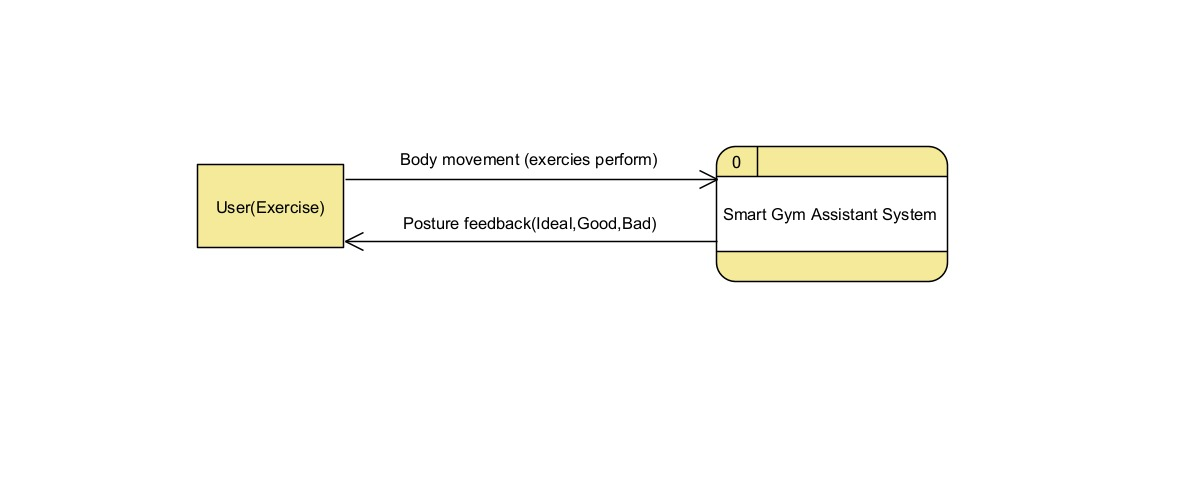
\includegraphics[width=0.82\textwidth]{Graphics/dfd0.jpeg}
\caption{Level 0 data flow diagram of the Smart Gym Assistant.}
\label{fig:system-design-dfd0}
\end{figure}

The Level 1 data flow diagram in Figure~\ref{fig:system-design-dfd} shows how data
moves through the complete system. The user provides exercise and posture labels in
collection mode, while the two MPU6050 sensors provide motion readings. The ESP32
collects and preprocesses these readings before either uploading labeled batches to
the FastAPI service or performing local KNN prediction. The service stores collection
data and exposes the latest live result to the browser dashboard.

\begin{figure}[H]
\centering
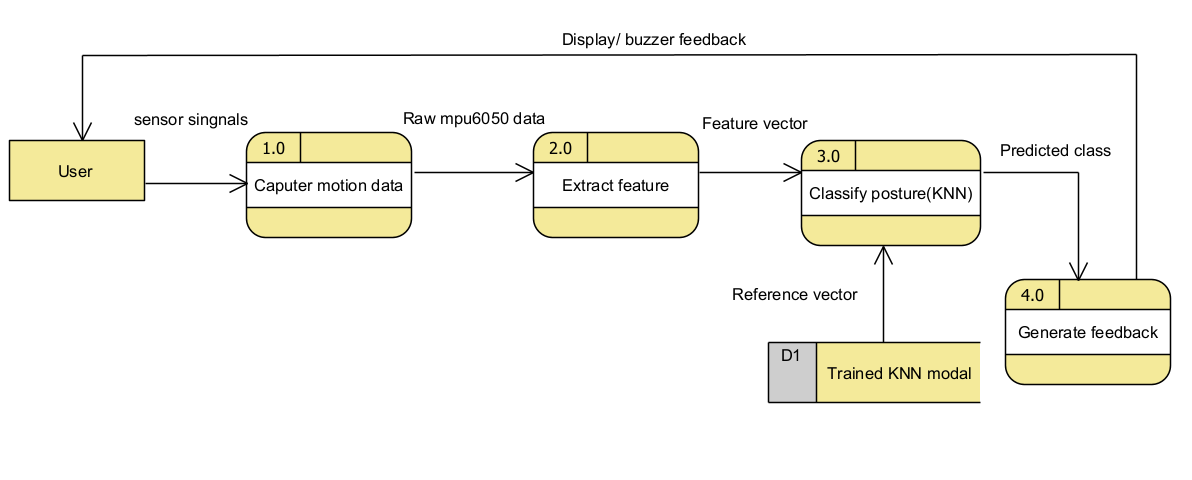
\includegraphics[width=0.88\textwidth]{Graphics/dfdlevel1.png}
\caption{Level 1 data flow diagram of the Smart Gym Assistant.}
\label{fig:system-design-dfd}
\end{figure}

This separation keeps raw training data distinct from live predictions. It also
allows the ESP32 to continue making time-sensitive decisions locally while the
server handles storage and web monitoring.

\section{Use-Case Diagram}
Figure~\ref{fig:system-design-usecase} presents the main interactions between the
user and the Smart Gym Assistant. The user can configure the exercise and posture,
collect labeled sensor data, start live monitoring, and observe exercise, posture,
confidence, and repetition results. The system performs sensing, classification,
feedback, data storage, and dashboard updates in response to these actions.

\begin{figure}[H]
\centering
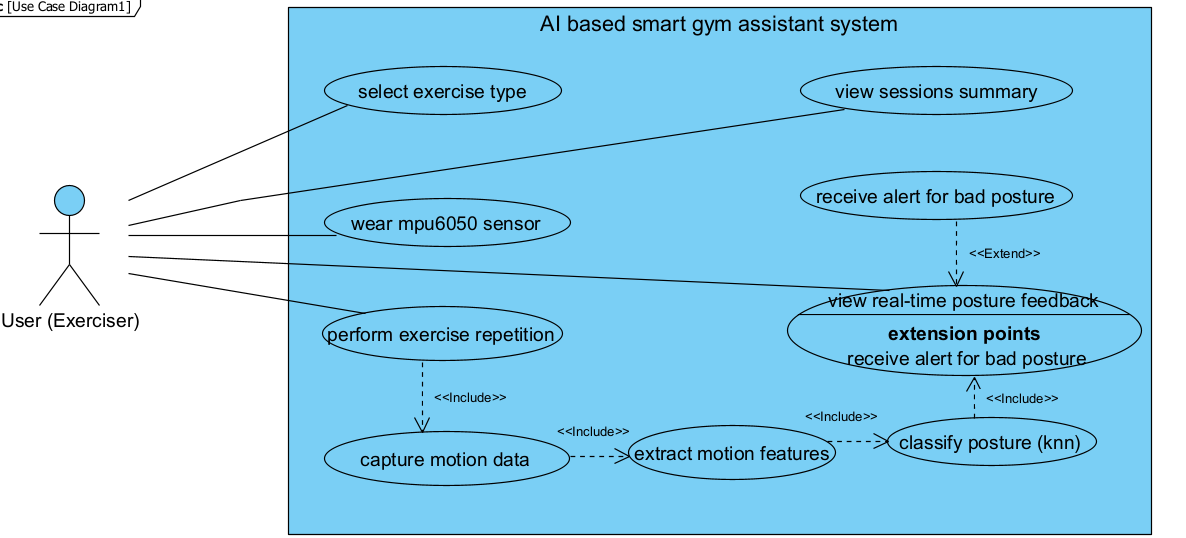
\includegraphics[width=0.82\textwidth]{Graphics/usecasediagram.png}
\caption{Use-case diagram of the Smart Gym Assistant.}
\label{fig:system-design-usecase}
\end{figure}

The use cases reflect the two operating modes. Collection mode is intended for
building the labeled dataset, whereas live mode is intended for real-time exercise
and posture feedback.

\section{Sequence Diagram}
The sequence diagram in Figure~\ref{fig:system-design-sequence} describes the order
of communication among the user, sensors, ESP32, FastAPI service, and dashboard.
During collection, the ESP32 gathers a complete batch and sends it to the API for
validation and storage. During live monitoring, it classifies the batch locally,
updates the OLED and buzzer, and publishes the latest result for the dashboard.

\begin{figure}[H]
\centering
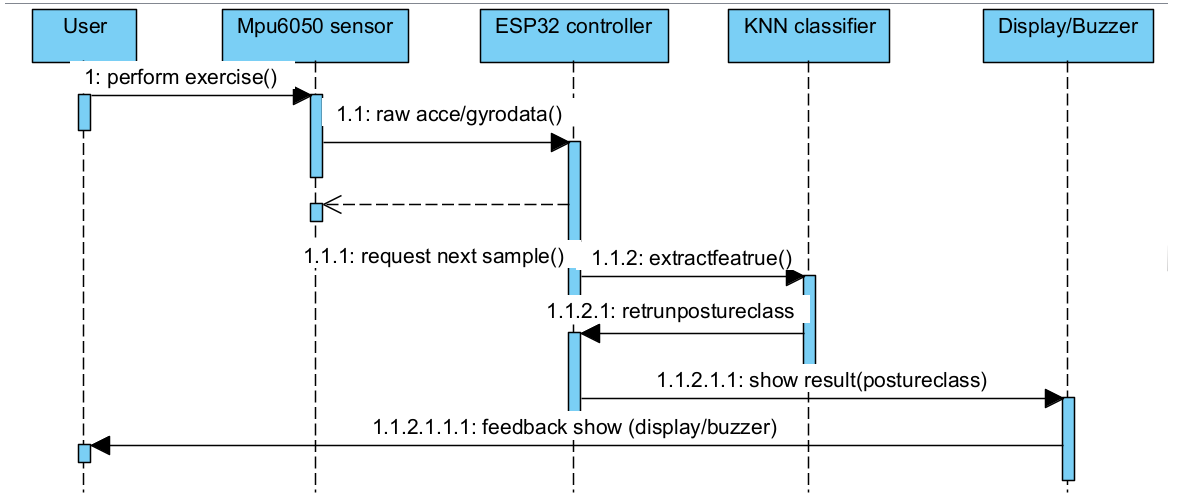
\includegraphics[width=0.88\textwidth]{Graphics/sequencediagram.png}
\caption{Sequence diagram for collection and live monitoring.}
\label{fig:system-design-sequence}
\end{figure}

The sequence emphasizes that sensor acquisition and inference occur on the ESP32,
while the FastAPI service provides storage and monitoring support. This arrangement
reduces dependence on network response time for immediate local feedback.

\section{Activity Diagram}
Figure~\ref{fig:system-design-activity} represents the operational workflow of the
system. The process begins with initialization and sensor setup, followed by mode
selection. In collection mode, labeled samples are buffered and uploaded. In live
mode, the buffered samples are standardized, classified with KNN, and converted into
exercise, posture, confidence, and repetition feedback. The workflow then repeats
for the next batch while the system remains active.

\begin{figure}[H]
\centering
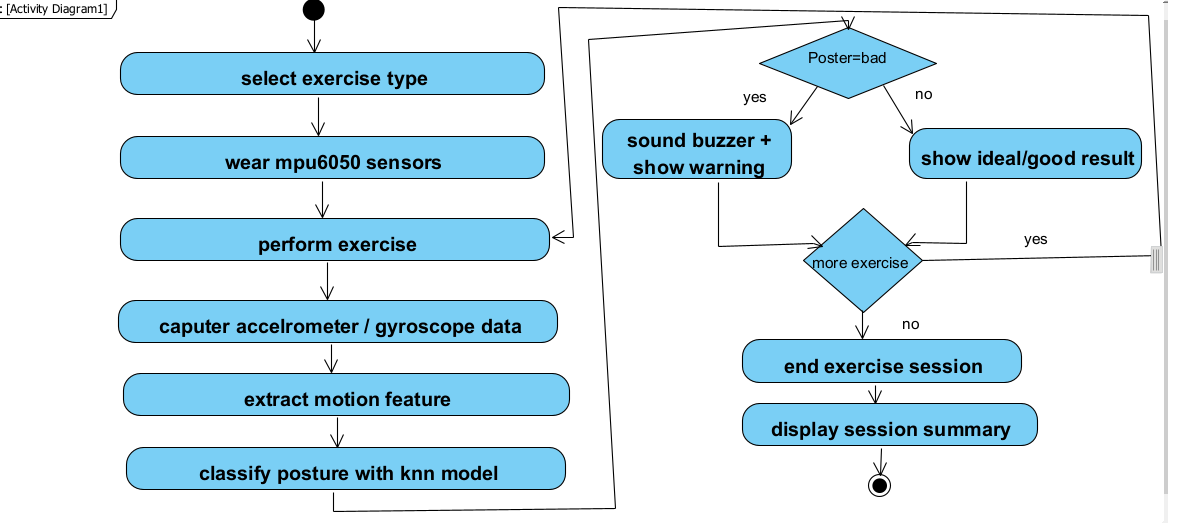
\includegraphics[width=0.82\textwidth]{Graphics/activity.png}
\caption{Activity diagram of the Smart Gym Assistant workflow.}
\label{fig:system-design-activity}
\end{figure}

The activity model also shows the control decisions that prevent collection and live
operation from being mixed. This supports reliable labeling and makes the system
behavior easier to test.

\section{Class Diagram}
The class diagram in Figure~\ref{fig:system-design-class} summarizes the logical
software structure. Sensor and buffer components provide motion samples, the KNN
model performs classification, and the feedback components update the OLED and
buzzer. Wi-Fi and API components handle communication with FastAPI, while the
repetition counter and dashboard data represent the user-visible results.

\begin{figure}[H]
\centering
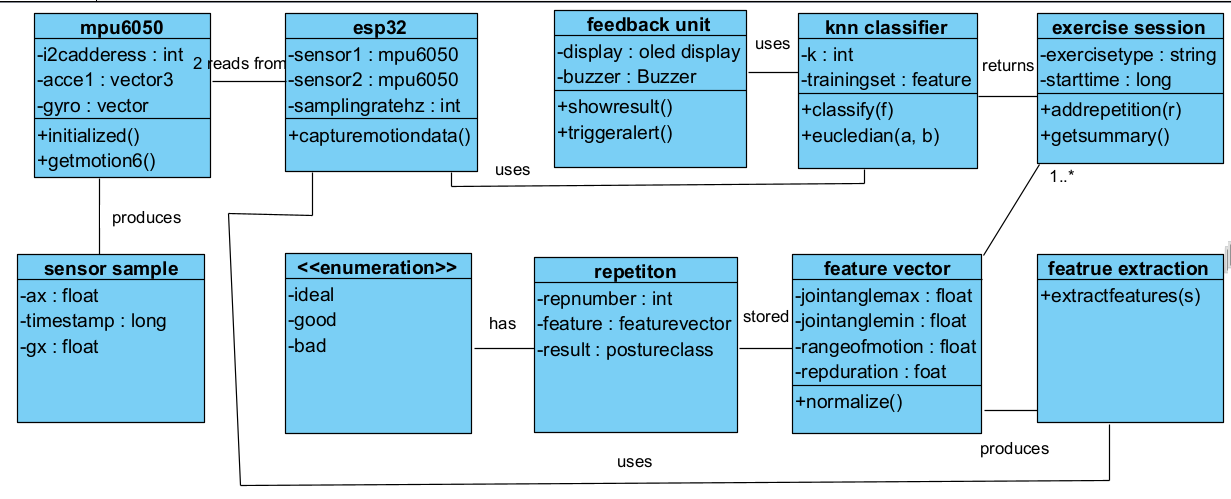
\includegraphics[width=0.88\textwidth]{Graphics/classdiagram.png}
\caption{Class diagram of the Smart Gym Assistant software structure.}
\label{fig:system-design-class}
\end{figure}

Although the firmware is implemented in embedded C++, the class diagram is a
logical representation of its modules and responsibilities. It shows how the
components cooperate without requiring the implementation to use a large software
framework.
